\PassOptionsToPackage{unicode}{hyperref}
\PassOptionsToPackage{hyphens}{url}
\PassOptionsToPackage{dvipsnames,svgnames,x11names,table}{xcolor}
%
\documentclass[english,paper=a4,captions=tableheading]{scrartcl}
\usepackage{microtype}
\usepackage{ragged2e}
\RaggedRight
\usepackage[text=cicero]{lipsum}
\usepackage{amsmath,amssymb}
\usepackage[sfdefault,type1]{librefranklin}

\makeatletter
\@ifundefined{KOMAClassName}{% if non-KOMA class
  \IfFileExists{parskip.sty}{%
    \usepackage{parskip}
  }{% else
    \setlength{\parindent}{0pt}
    \setlength{\parskip}{6pt plus 2pt minus 1pt}}
}{% if KOMA class
  \KOMAoptions{parskip=half}}
\makeatother

\usepackage{xcolor}
\definecolor{default-linkcolor}{HTML}{A50000}
\definecolor{default-filecolor}{HTML}{A50000}
\definecolor{default-citecolor}{HTML}{4077C0}
\definecolor{default-urlcolor}{HTML}{4077C0}
\definecolor{some-blue}{HTML}{0C2D82}
\IfFileExists{xurl.sty}{\usepackage{xurl}}{} % add URL line breaks if available
\IfFileExists{bookmark.sty}{\usepackage{bookmark}}{\usepackage{hyperref}}
\hypersetup{
  pdftitle={THE MAIN TITLE},
  pdfauthor={THE AUTHOR},
  pdflang={en},
  pdfsubject={Markdown},
  pdfkeywords={Markdown, Trial},
  hidelinks,
  breaklinks=true,
  pdfcreator={some pub pipe v2022.4.12}}
\urlstyle{same} % disable monospaced font for URLs
\usepackage[left=2cm,top=1cm,right=2cm,bottom=0.8cm,head=18.30666pt,includehead=true,includefoot=true,centering]{geometry}
\usepackage{listings}
\usepackage{longtable,booktabs,array}
\usepackage{calc} % for calculating minipage widths
% Correct order of tables after \paragraph or \subparagraph
\usepackage{etoolbox}
\usepackage{pagecolor}
\usepackage{afterpage}
\usepackage{tikz}
\usepackage{setspace}

\usepackage{graphicx}
\usepackage{svg}
\providecommand{\tightlist}{%
  \setlength{\itemsep}{0pt}\setlength{\parskip}{0pt}}

\definecolor{heading-color}{RGB}{40,40,40}
\addtokomafont{section}{\color{heading-color}}
% When using the classes report, scrreprt, book, scrbook or memoir, uncomment the following line.
%\addtokomafont{chapter}{\color{heading-color}}

\usepackage[headsepline,footsepline]{scrlayer-scrpage}

\newpairofpagestyles{over-engineered-header-footer}{
  \clearpairofpagestyles
  \ihead*{LEFT HEAD TITLE}
  \chead*{CENTER HEAD DATA}
  \ohead*{\includesvg[height=0.5cm]{logo}}
  \ifoot*{LEFT FOOT DATA}
  \cfoot*{CENTER FOOT DATA}
  \ofoot*{\thepage}
  \addtokomafont{pageheadfoot}{\upshape}
}
\pagestyle{over-engineered-header-footer}

\begin{document}

\begin{titlepage}
\newgeometry{top=1cm, right=4cm, bottom=0.8cm, left=4cm}
\tikz[remember picture,overlay] \node[inner sep=0pt] at (current page.center){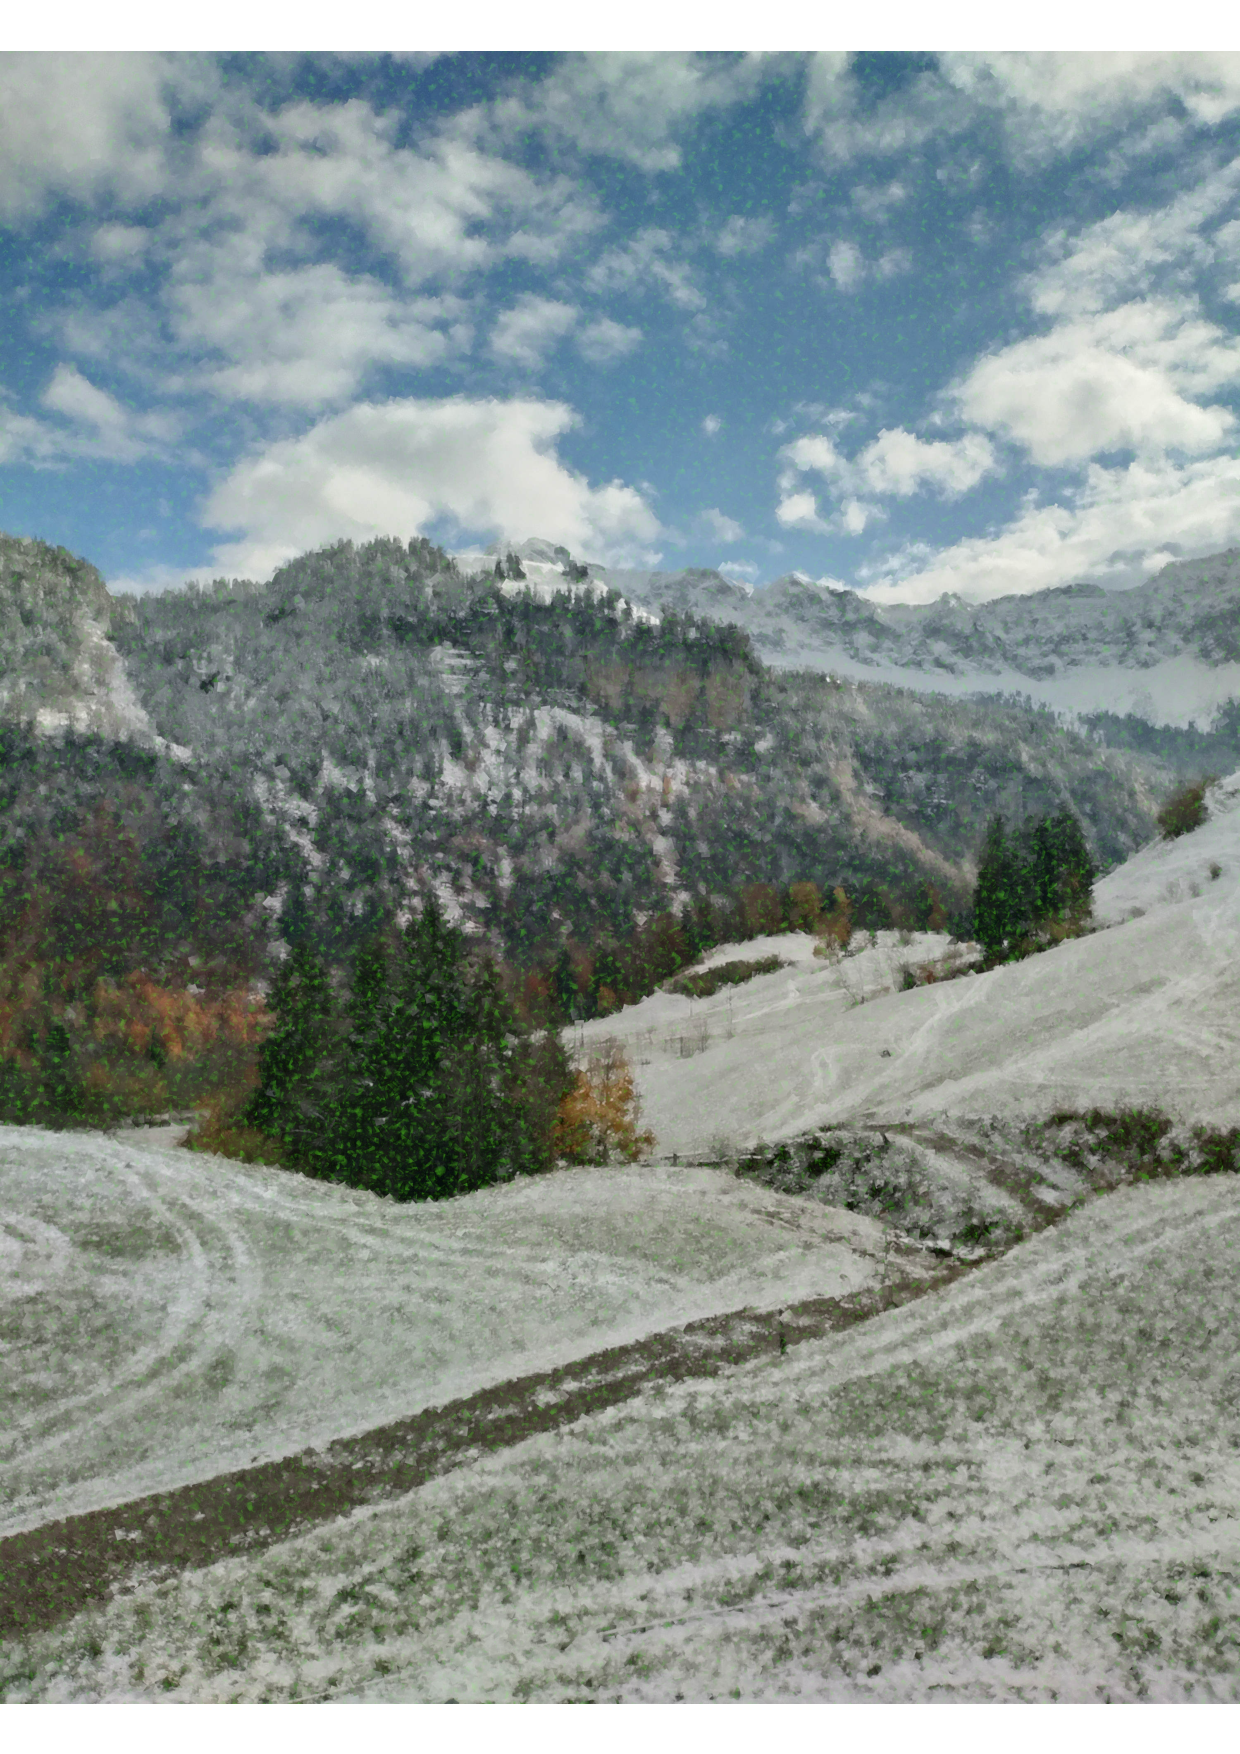
\includegraphics[width=\paperwidth,height=\paperheight]{bg.pdf}};
\newcommand{\colorRule}[3][black]{\textcolor[HTML]{#1}{\rule{#2}{#3}}}
\begin{flushleft}
\noindent
\\[-1em]
\color[HTML]{ffffff}
\makebox[0pt][l]{\colorRule[360049]{1.3\textwidth}{0pt}}
\par
\noindent

% The titlepage with a background image has other text spacing and text size
{
  \setstretch{2}
  \vskip 14em
  \noindent {\color[HTML]{000000} \Huge \hskip -2.8em \textbf{\textsf{\mbox{THE}\nolinebreak\ \mbox{DOC}\nolinebreak\ \mbox{MAIN}\nolinebreak\ \mbox{TITLE}}}}
  \vskip 1em
  {\color[HTML]{000000} \LARGE \hskip -4em \textsf{THE SUBTITLE}}
  \vskip 5em  %%%% was 2 or so
  \vfill
}

\end{flushleft}
\end{titlepage}
\restoregeometry
\pagenumbering{arabic} 

%%
%% end titlepage
%%
\mbox{}\vskip 4em

\begin{longtable}[]{|
  >{\raggedright\arraybackslash}p{(\columnwidth - 12\tabcolsep) * \real{0.1700}}|
  >{\centering\arraybackslash}p{(\columnwidth - 12\tabcolsep) * \real{0.2850}}|
  >{\centering\arraybackslash}p{(\columnwidth - 12\tabcolsep) * \real{0.2850}}|
  >{\centering\arraybackslash}p{(\columnwidth - 12\tabcolsep) * \real{0.2850}}|}
\hline
\begin{minipage}[b]{\linewidth}\raggedright
\ \mbox{\textbf{COL HEAD LEG}}
\end{minipage} & \begin{minipage}[b]{\linewidth}\centering
\mbox{\textbf{COL1}}
\end{minipage} & \begin{minipage}[b]{\linewidth}\centering
\mbox{\textbf{COL2}}
\end{minipage} & \begin{minipage}[b]{\linewidth}\centering
\mbox{\textbf{COL3}}
\end{minipage} \\
\hline
\ \mbox{\textbf{ROW1 LEG}} & Author & Reviewer & Approver \\
\hline
\ \mbox{\textbf{ROW2 LEG}} & Some Author & Some Reviewer & Some Approver \\
\hline
\ \mbox{\textbf{ROW3 LEG}}\newline & & & \\
\hline
\end{longtable}

\mbox{}\vskip 14em
\hypertarget{change-log}{%
\section*{Change Log}\label{change-log}}

\begin{longtable}[]{|
  >{\centering\arraybackslash}p{(\columnwidth - 6\tabcolsep) * \real{0.0600}}|
  >{\centering\arraybackslash}p{(\columnwidth - 6\tabcolsep) * \real{0.1600}}|
  >{\centering\arraybackslash}p{(\columnwidth - 6\tabcolsep) * \real{0.1600}}|
  >{\raggedright\arraybackslash}p{(\columnwidth - 6\tabcolsep) * \real{0.5800}}|}
\hline
\begin{minipage}[b]{\linewidth}\centering
\textbf{Iss.}
\end{minipage} & \begin{minipage}[b]{\linewidth}\centering
\textbf{Author}
\end{minipage} & \begin{minipage}[b]{\linewidth}\centering
\textbf{Date}
\end{minipage} & \begin{minipage}[b]{\linewidth}\raggedright
\textbf{Description}
\end{minipage} \\
\hline
 42 & Some Author & 2022-04-12 & Initial issue \\
\hline
\end{longtable}

\hypertarget{proprietary-information}{%
\section*{Proprietary Information}\label{proprietary-information}}

Legal statement.

\newpage
\renewcommand*\contentsname{Table of Contents}
{
\setcounter{tocdepth}{2}
\tableofcontents
}
\listoftables
\newpage
\listoffigures
\newpage

\hypertarget{scope}{%
\section{Scope}\label{scope}}

This named document (ND) does define things.
We can also read three paragraphs of blind text (to dissect the ragged right layout):

\lipsum[2-3][1-2]

\lipsum[3-9][4-8]

\lipsum[1-2][3-4]

The document describes in detail the following:

\begin{itemize}
\tightlist
\item
  Things
\item
  We
\item
  Do
\end{itemize}

We also do things in order (sequence) like so:

\begin{enumerate}
\def\labelenumi{\arabic{enumi}.}
\tightlist
\item
  First
\item
  Second
\item
  Third
\item
  Fourth
\end{enumerate}

These four technical things are fun and important at the same time.

\hypertarget{other-section}{%
\section{Other Section}\label{other-section}}

This does all the right thing. For more details cf.~{[}OTHER FAKE LINK{]}
or \hyperref[acronyms]{\color{some-blue}Acronyms}.

\hypertarget{some-subsection}{%
\subsection{Some Subsection}\label{some-subsection}}

No deviations from the section.

\hypertarget{some-subsubsection}{%
\subsubsection{Some Subsubsection}\label{some-subsubsection}}

Every subsection may have a subsubsection.

\textbf{NOTE}: some soft notes without dedicated format element.

A link: \href{https://example.com}{\color{some-blue}Example domain}

\newpage
\hypertarget{section-on-new-page}{%
\section{Section on new Page}\label{section-on-new-page}}

The facts conveyed are per the following diagram:

%TODO: find a better place upstairs where not overridden but off of the content
\setcapwidth[c]{.3\textwidth}
\setcapindent{0pt}
\addtokomafont{caption}{\centering}

\begin{figure}
\centering

\includegraphics[width=0.93\linewidth]{images/facts.png}
\caption{\color{heading-color}\textbf{Facts}}
\end{figure}

\hypertarget{acronyms}{%
\section{Acronyms}\label{acronyms}}

\begin{small}
  \begin{longtable}[]{|
    >{\raggedright\arraybackslash}p{(\columnwidth - 6\tabcolsep) * \real{0.2500}}|
    >{\raggedright\arraybackslash}p{(\columnwidth - 6\tabcolsep) * \real{0.7500}}|}
  \hline
\textbf{Term} & \textbf{Description} \\
\hline
API & Application Programming Interface \\
\hline
PC & Personal Computer \\
\hline
\end{longtable}
\end{small}
\end{document}
